% Chapter 3
\chapter{System Architecture and Methodology}
\label{ch:methodology}

This chapter describes how the project turns five raw PKDD'99 tables into a scored loan portfolio. The work is organised as an offline analytical pipeline with four layers: data assembly, feature engineering, modelling, and serving. Each layer writes a durable artifact, so a result shown in the report or the dashboard can be traced back to a file produced by an earlier stage.

\section{Pipeline Overview}
\label{sec:pipeline-overview}

Figure~\ref{fig:architecture} shows the end-to-end flow. The data layer reads the loan, transaction, client, account, and disposition tables. The feature layer builds one row per loan using only transactions dated before the loan was granted. The modelling layer trains six classifiers under two imbalance settings, tunes them, and evaluates them with a held-out split and repeated cross-validation. The serving layer exposes the resulting metrics, feature importances, risk scores, and mined patterns through a Streamlit console.

\begin{figure}[H]
    \centering
    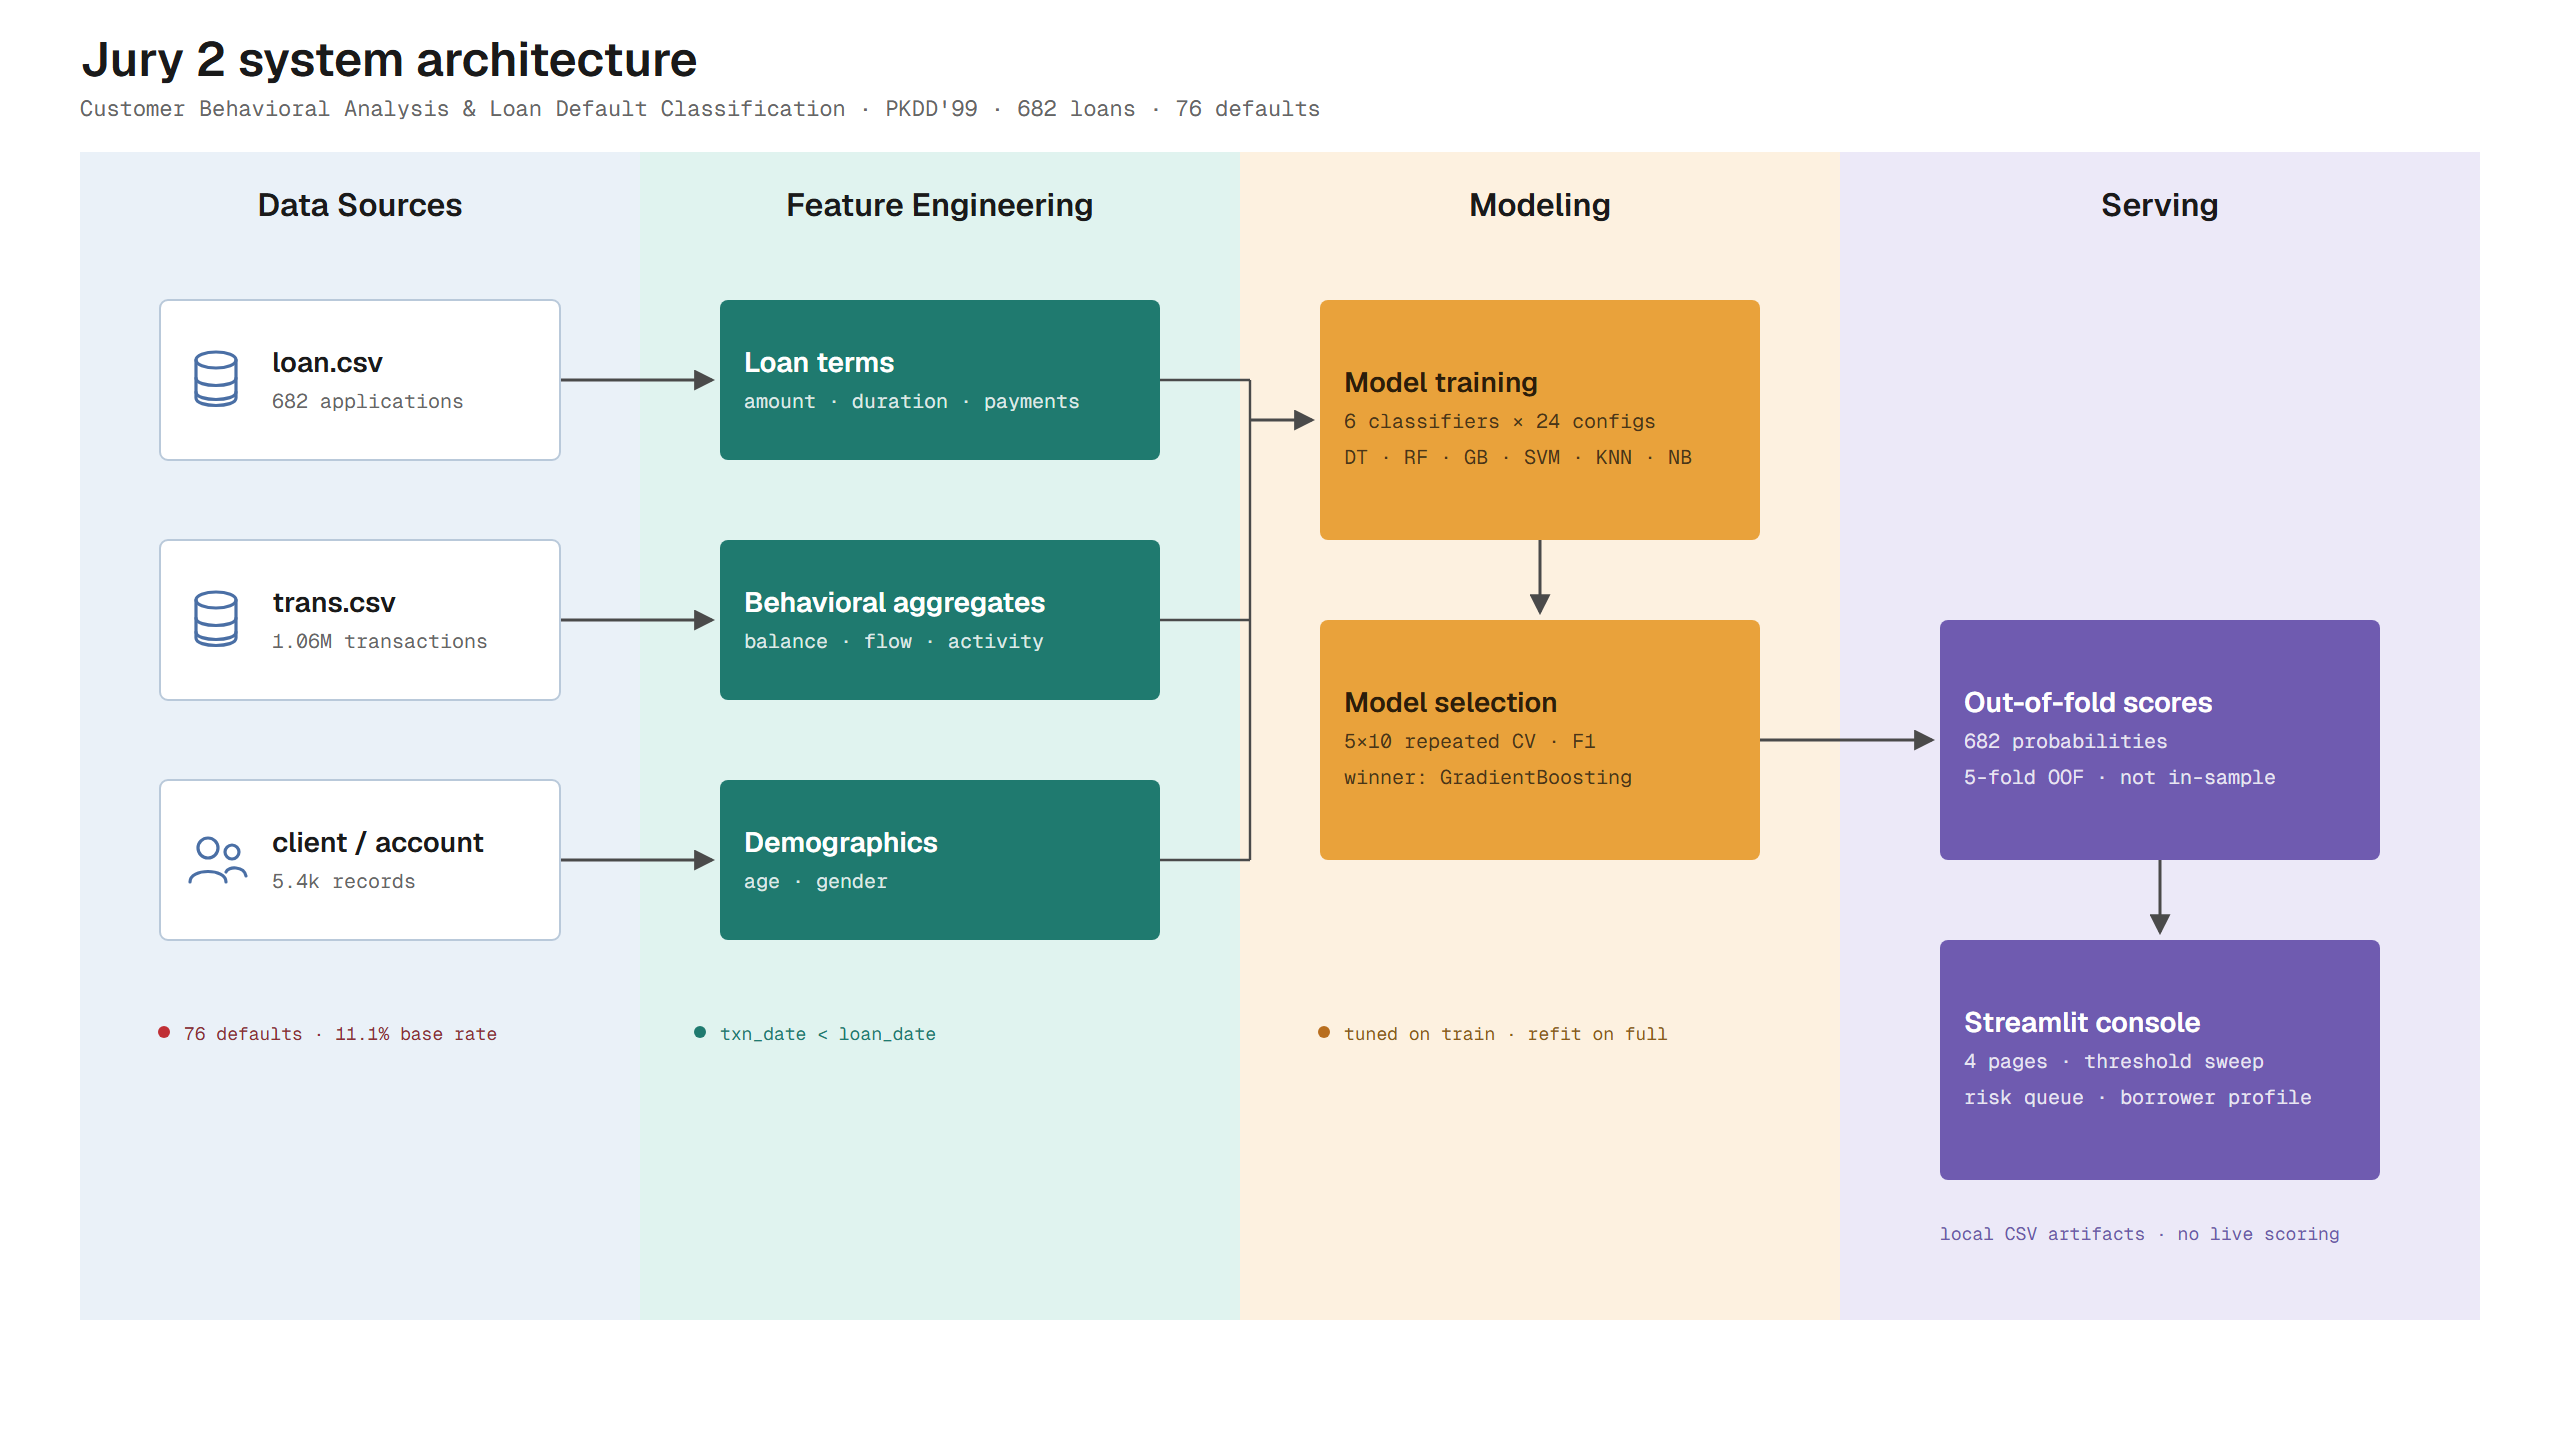
\includegraphics[width=\textwidth]{jury2-architecture.png}
    \caption{End-to-end architecture of the loan default classification project. The pipeline is batch-oriented: each stage reads files from the previous stage and writes a versioned artifact.}
    \label{fig:architecture}
\end{figure}

The design keeps the analytical work separate from the presentation work. Notebooks produce CSV and PNG artifacts under \texttt{outputs/}; the dashboard only reads those artifacts and does not retrain a model when a page is opened. This makes the reported numbers stable and allows the console to run on a machine without the full training environment.

\section{Technology Stack}
\label{sec:technology-stack}

The implementation uses open-source Python tools. Table~\ref{tab:stack} lists the main components and their responsibilities.

\begin{table}[H]
    \centering
    \caption{Tools used in the project and their roles.}
    \label{tab:stack}
    \begin{tabularx}{\textwidth}{@{}lX@{}}
        \toprule
        \textbf{Tool} & \textbf{Role in the project} \\
        \midrule
        Python 3.13.5 & Main programming language for all notebooks and scripts. \\
        pandas 2.2.3 & Reading the CSV extracts, joining tables, and building loan-level features. \\
        NumPy 2.2.4 & Numeric operations and array handling inside pandas and scikit-learn. \\
        scikit-learn 1.7.0 & Classifiers, pipelines, scaling, cross-validation, and hyperparameter search. \\
        imbalanced-learn 0.14.2 & SMOTE oversampling inside the modelling pipeline. \\
        matplotlib 3.10.3 & Base plotting for the figures in this report. \\
        seaborn 0.13.2 & Distribution, box, and correlation plots. \\
        mlxtend & Apriori and FP-Growth pattern mining. \\
        Jupyter Notebook & Literate analysis; notebooks are executed in order with nbconvert. \\
        Streamlit & Interactive review console for the exported results. \\
        \bottomrule
    \end{tabularx}
\end{table}

The versions shown for the core Python libraries are the ones recorded for the analysis environment. The notebooks also rely on the standard library modules \texttt{pathlib}, \texttt{json}, and \texttt{warnings}. No database server or distributed compute engine is required; the largest table, \texttt{trans.csv}, has 1,056,320 rows and fits comfortably in memory on a laptop.

\section{Pipeline Stages}
\label{sec:pipeline-stages}

\subsection{Data Assembly}
The five source files are loaded with explicit column types where needed. The disposition table links clients to accounts. A client can be an owner or a disbursent, and the same account can have more than one client. Only rows with \texttt{disp.type = OWNER} are used, because the loan is associated with the account owner rather than with every person who can operate the account. The account table supplies the district, the client table supplies the birth number, and the loan table supplies the target and the loan terms.

\subsection{Cleaning and Target Construction}
Dates in the source files use the \texttt{\%y\%m\%d} format and are parsed to a common date type. The loan status is mapped to a binary target: status A (finished, no problems) and C (running, no problems) become good loans, while status B (finished with problems) and D (running with problems) become defaults. The resulting label is imbalanced at roughly one default for every nine good loans, which shapes the rest of the methodology.

\subsection{Feature Engineering}
For every loan, the transaction table is filtered to records dated strictly before the loan date. The filtered history is aggregated into 13 behavioural features that describe activity volume, cash flow, balance level, and account history. Loan amount, duration, and payment are taken from the loan record. Age, gender, and district are taken from the client and account records. The feature table is written once and reused by all later notebooks, so the modelling code cannot accidentally see transactions after the loan date.

\subsection{Model Training and Evaluation}
The modelling notebook reads the feature table, creates a stratified train/test split, and trains the six classifiers described in Chapter~\ref{ch:literature}. Each classifier is run once with its default hyperparameters and once with SMOTE applied inside the pipeline. Hyperparameters are then searched on the training split only. The tuned and untuned configurations are compared with repeated stratified cross-validation, and the selected configuration is refit on the full training split.

\subsection{Artifact Generation and Serving}
The modelling stage writes metrics tables, curve data, confusion matrices, feature importances, the fitted model, and out-of-fold risk scores. The pattern mining script writes itemsets and rules. The Streamlit application reads these files and presents four pages: model comparison, an explanation of the selected model, a review queue, and the pattern mining results. The review queue is a prioritisation aid, not an automatic approval or rejection system.

\section{Input and Output Specification}
\label{sec:io}

The pipeline has two interfaces. The first is the file boundary between stages: each stage reads the artifact written by the previous stage and writes a new one. The second is the model boundary: a loan is passed to the fitted pipeline as a vector of 18 numeric features, and the pipeline returns a score. Table~\ref{tab:io} lists both.

\begin{table}[H]
    \centering
    \caption{Inputs and outputs at each stage of the pipeline.}
    \label{tab:io}
    \small
    \begin{tabularx}{\textwidth}{@{}>{\raggedright\arraybackslash}p{2.8cm} X X@{}}
        \toprule
        \textbf{Stage} & \textbf{Input} & \textbf{Output} \\
        \midrule
        Data assembly & \texttt{loan.csv}, \texttt{trans.csv}, \texttt{client.csv}, \texttt{account.csv}, \texttt{disp.csv} & Clean loan base table with 682 rows and the account and client keys. \\
        \addlinespace
        Feature engineering & Loan base table and transactions dated before each loan & \texttt{data/loan\_features.csv}: 682 rows, 27 columns, 18 model features. \\
        \addlinespace
        Training & Feature table, fixed seed 42, and the stratified train/test split & Fitted pipeline \texttt{best\_GradientBoosting\_baseline\_tuned.pkl}; metric, tuning, and curve tables. \\
        \addlinespace
        Scoring & Fitted pipeline and one loan feature vector & Default score and rank for the loan; 682 out-of-fold scores in \texttt{loan\_risk\_dashboard.csv}. \\
        \addlinespace
        Presentation & Exported CSV and PNG artifacts & Streamlit pages for comparison, explanation, review queue, and patterns. \\
        \bottomrule
    \end{tabularx}
\end{table}

At the model boundary, the input is the 18 features listed in Table~\ref{tab:model-features}. The output is a continuous score from \texttt{predict\_proba}, treated as a rank rather than a calibrated probability. A binary label is produced only after a threshold is applied, and the review queue deliberately uses the rank so that no single cutoff is presented as an approval rule. The five raw CSV files are the only external inputs; there is no database, API, or manual data entry in the pipeline.

\section{Leakage Controls}
\label{sec:leakage-controls}

Leakage is the main methodological risk in a project that combines account history with a future outcome. Four controls are applied throughout.

\begin{enumerate}
    \item \textbf{Time cutoff.} A transaction enters a loan's feature vector only if its date is strictly earlier than the loan date. The comparison is strict, so transactions booked on the same day as the loan are excluded.
    \item \textbf{Pipeline-contained preprocessing.} Scaling and SMOTE are steps inside a scikit-learn pipeline. During cross-validation they are fitted on the training fold and applied to the validation fold, never fitted on the full dataset before the split.
    \item \textbf{Training-only tuning.} The randomized search sees only the training partition. The held-out test partition is used once, for the final comparison table, and does not influence the choice of model or hyperparameters.
    \item \textbf{Target-free segmentation.} The KMeans segmentation used in the exploratory analysis is fitted on behavioural and loan variables with the default label excluded. Segment default rates are computed after clustering and are therefore an honest description of the groups, not an input to them.
\end{enumerate}

The transaction history is also left-censored in a way that should be stated plainly. The extract begins in 1993, so a loan granted early in the period has a shorter observable history than a loan granted in 1998. The feature \texttt{months\_active} records the span between the first observed transaction and the loan date, which lets the model distinguish a genuinely quiet account from one with little recorded history.

\section{Evaluation Protocol}
\label{sec:evaluation-protocol}

The evaluation follows four steps.

\begin{enumerate}
    \item \textbf{Held-out comparison.} A stratified 75/25 split produces 511 training loans and 171 test loans, with 57 and 19 defaults respectively. All twelve model/setting combinations are trained on the training partition and scored on the test partition. This gives a first, readable comparison under default hyperparameters.
    \item \textbf{Hyperparameter search.} For each model and imbalance setting, \texttt{RandomizedSearchCV} samples up to 30 parameter combinations and scores them with F1 on an inner five-fold stratified cross-validation of the training partition. F1 is used because accuracy is dominated by the majority class at an 11\% default rate.
    \item \textbf{Repeated cross-validation.} The default and tuned versions of all twelve configurations are evaluated with \texttt{RepeatedStratifiedKFold(5, 10)}: five folds repeated ten times, giving 50 F1 estimates per configuration. The mean and standard deviation are reported. This step is the basis for selecting the final model, because a single 171-loan test set is too small to separate close contenders.
    \item \textbf{Final refit and review scores.} The selected configuration is refit on the full training partition and saved. Separately, five-fold out-of-fold probabilities are generated for all 682 loans for the review queue. Those probabilities are out-of-sample by construction and are not the resubstitution scores of the final model.
\end{enumerate}

Average precision and ROC-AUC are reported alongside F1. Accuracy and precision are included for completeness, but they are not used for selection: a model can reach high accuracy by predicting the majority class, and precision alone says nothing about how many defaults are missed.

\section{Reproducibility}
\label{sec:reproducibility}

The analysis is organised as five notebooks that are executed in order:

\begin{enumerate}
    \item \texttt{01\_preprocessing.ipynb}: loads and cleans the source tables, resolves the owner relationship, and constructs the target.
    \item \texttt{02\_features.ipynb}: builds the pre-loan behavioural features and writes \texttt{data/loan\_features.csv}.
    \item \texttt{03\_eda.ipynb}: produces the exploratory figures and summary statistics.
    \item \texttt{04\_modeling.ipynb}: runs the single-split comparison, the hyperparameter search, the repeated cross-validation, the final refit, and the out-of-fold scores.
    \item \texttt{05\_segmentation.ipynb}: clusters loans without the target and profiles the resulting segments.
\end{enumerate}

A fixed random seed of 42 is used for the train/test split, the KMeans initialisation, and the randomized searches. The notebooks contain assertion cells for row counts, class counts, missing values, and the absence of post-loan transactions in the feature table. These checks turn silent data drift into a visible failure. The pattern mining step is kept in \texttt{tools/pattern\_mining.py} because it is a short, self-contained script rather than an interactive analysis.

The next chapter describes the data preparation in detail, including the exact feature definitions and the checks applied before modelling.
